
\documentclass[11pt,compress,t,notes=noshow]{beamer}

\usepackage[english]{babel}
\usepackage{dsfont}
\newcommand\bmmax{2}
\usepackage{bm}
\usepackage{bbm}
\usepackage{verbatim}
\usepackage{amsmath}
\usepackage{amsfonts}
\usepackage{csquotes}
\usepackage{multirow}
\usepackage{longtable}
\usepackage{enumerate}
\usepackage[absolute,overlay]{textpos}
\usepackage{psfrag}
\usepackage{algorithm}
\usepackage{algorithmicx}
\usepackage{algpseudocode}
\usepackage{eqnarray}
\usepackage{multimedia}
\usepackage{media9}
\usepackage{arydshln}
\usepackage{tabularx}
\usepackage{placeins}
\usepackage{tikz}
\usepackage{setspace}
\usepackage{wrapfig}
\usepackage{tcolorbox}
\usepackage[export]{adjustbox}
\usepackage{siunitx}
\usetikzlibrary{shapes,arrows,automata,positioning,calc}
\tikzset{
  %Define standard arrow tip
  >=stealth',
  %Define style for boxes
  punkt/.style={
    rectangle,
    rounded corners,
    draw=black, very thick,
    text width=6.5em,
    minimum height=2em,
    text centered},
  % Define arrow style
  pil/.style={
    ->,
    thick,
    shorten <=2pt,
    shorten >=2pt,}
}
\usepackage{subfig}

%new environments

\newenvironment{vbframe}  %frame with breaks and verbatim
{
 \begin{frame}[containsverbatim,allowframebreaks]
}
{
\end{frame}
}

\newenvironment{vframe}  %frame with verbatim without breaks (to avoid numbering one slided frames)
{
 \begin{frame}[containsverbatim]
}
{
\end{frame}
}

\newenvironment{blocki}[1]   % itemize block
{
 \begin{block}{#1}\begin{itemize}
}
{
\end{itemize}\end{block}
}

\newenvironment{fragileframe}[2]{  %fragile frame with framebreaks
\begin{frame}[allowframebreaks, fragile, environment = fragileframe]
\frametitle{#1}
#2}
{\end{frame}}


\newcommand{\myframe}[2]{  %short for frame with framebreaks
\begin{frame}[allowframebreaks]
\frametitle{#1}
#2
\end{frame}}

\newcommand{\remark}[1]{
  \textbf{Remark:} #1
}

%%%%%%%%%%%%%%%%%%%%%%%%%%%%%%%%%%%%%%%%%%%%%%%%%%%%%%%%%%%%%%%%%%%%%%%%%%%%%%%

% basic latex stuff
\newcommand{\pkg}[1]{{\fontseries{b}\selectfont #1}} %fontstyle for R packages
\newcommand{\lz}{\vspace{0.5cm}} %vertical space
\newcommand{\dlz}{\vspace{1cm}} %double vertical space
\newcommand{\oneliner}[1] % Oneliner for important statements
{\begin{block}{}\begin{center}\begin{Large}#1\end{Large}\end{center}\end{block}}


%\usetheme{lmu-lecture}
\usepackage{../style/lmu-lecture}

\let\code=\texttt
\let\proglang=\textsf

\setkeys{Gin}{width=0.9\textwidth}



\title{Deep Learning}
\author{David Rügamer}
\institute{Department of Statistics -- LMU Munich}
\date{Winter Semester 2021}

\setbeamertemplate{frametitle}{\expandafter\uppercase\expandafter\insertframetitle}

%\begin{document}
%\sloppy
%\end{document}


\input{../../latex-math/basic-math}
\input{../../latex-math/basic-ml}
\input{../../latex-math/ml-nn}

\begin{document}

\lecturechapter{1}{A Single Neuron}
\lecture{Deep Learning}


% SOURCE for animations: 
% --- 
% https://docs.google.com/presentation/d/1kLU5RxNlDq8ohJNSp6UmNu9Y4I6J1BWI2Ax5bOAASK0/edit
% --- 

%%%%%%%%%%%%%%%%%%%%%%%%%%%%%%%%%%%%%%%%%%%%%%%%%%%%%%%%%%%%%%%%%%

% \begin{frame} {Logistic Regression*}
%   \begin{itemize}
%     \item In order to better understand the types of functions that neural networks can represent, we begin by briefly examining a very simple machine learning algorithm: logistic regression. REWORD
%     \vspace{3mm}
%     \item In a binary classification task, the goal is to map an input $x$ to a binary target variable $y$.
%     \vspace{3mm}
%     \item It models y as {TODO}    
%       \begin{itemize}
%         \item Weights {TODO}
%         \item The bias term must not be confused with the statistical bias. It actually is an intercept parameter.
%     \item Logistic regression example {TODO}
%         \item Sigmoid function {TODO}
%       \end{itemize}
%   \end{itemize}
% \end{frame}

% \begin{frame} {Logistic Regression}
%   \begin{itemize}
%     \item Sigmoid function $$ \sigma(v) = \frac{1}{(1+\exp (-s \cdot v))} $$
%     <<echo=FALSE, fig.height=2.7>>=
% library(ggplot2)
% logfun = function(v, s) {
%   1 / (1 + exp(- s * v))
% }
% x = seq(-10, 10, 0.1)
% stretch = c(0.25, 1, 10)
% y = sapply(stretch, function(s) {
%   sapply(x, logfun, s = s)
% })
% df = data.frame(y = as.vector(y), x = rep(x, length(stretch)),
%   s = as.factor(rep(stretch, each = length(x))))
% 
% logfun.q = ggplot(df, aes(x = x, y = y, color = s)) + geom_line(size=1)
% logfun.q = logfun.q + scale_y_continuous(name = NULL)
% logfun.q = logfun.q + scale_x_continuous(name = NULL)
% logfun.q = logfun.q + theme(axis.title = element_text(size = 14L, face = "bold"),
%   plot.margin = unit(c(0, 0, 0, 0), "cm"))
% logfun.q
% @
%     \item \small{This "squashes" the output to be between 0 and 1.}
%   \end{itemize}
% \end{frame}
% 
% \begin{frame} {Logistic Regression}
%   \begin{itemize}
%   \item Some important properties of the sigmoidal logistic function include:
%   \item[]
%   \item[]
%   \begin{itemize}
%     \item limits: $$\lim_{v \to -\infty} \sigma(v) = 0 \text{ and } \lim_{v \to \infty} \sigma(v) = 1$$
%     \item the derivative for $s = 1$: $$\frac{\delta\sigma(v)}{\delta v}=\frac{\exp(v)}{(1+\exp(v))^2} = \sigma(v)(1-\sigma(v))$$
%     \item for any s: $$\sigma(v) \text{ is symmetrical in } (0, 0.5)$$
%   \end{itemize}
% \end{itemize}
% \end{frame}
% 
% \begin{frame} {Types of boundaries that can be learned}
%   \begin{itemize}
%     \item Different values of $\mathbf{w}$ and $b$ map to different linear decision boundaries separating the two classes.
%     \vspace{5mm}
%     \begin{figure}
%     \centering
%       \scalebox{1}{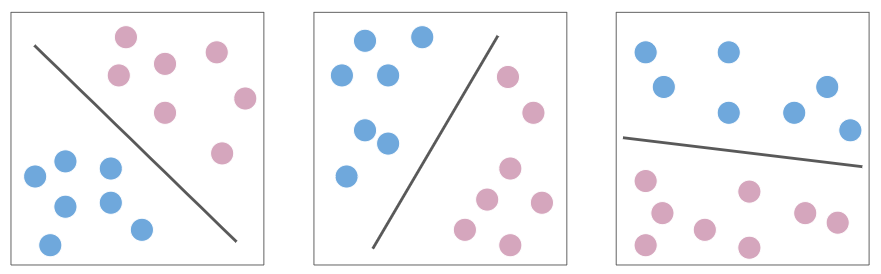
\includegraphics{plots/lin_bound.png}}
%   \end{figure}
%     \vspace{5mm}
%   Note: Only two dimensions pictured here
%   \end{itemize}
% \end{frame}
% 
% \begin{frame} {Types of boundaries that can be learned}
% \begin{itemize}
%     \item As already stated, the bias term must not be confused with the statistical bias.
%     \item It is actually an intercept parameter, which puts the decision boundary at the correct position in the learned space.
%     % Deeplearningbook page 110: This terminology derives from the point of view that the output of the transformation is biased toward being b in the absence of any input.
%   \end{itemize}
%     \begin{figure}
%       \centering
%         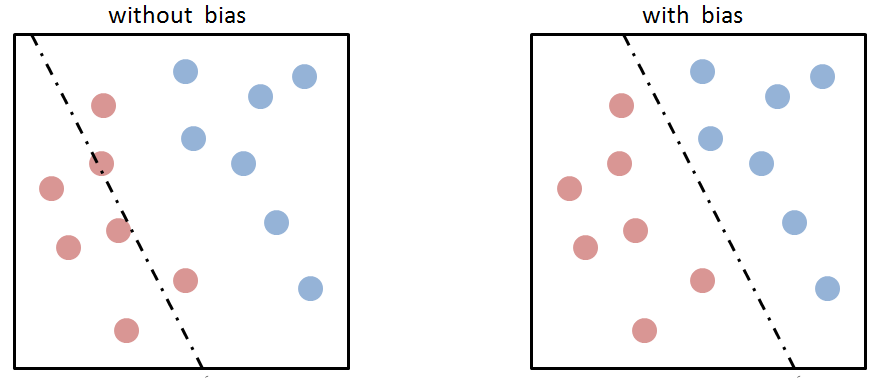
\includegraphics[width=8.5cm]{plots/bias.png}
%     \end{figure}
% \end{frame}


\begin{frame} {A Single Neuron}
  \begin{itemize}
    \vspace{5mm}
    \item In order to better understand the types of functions that neural networks can represent, let us begin with a very simple model: logistic regression.
    \item Recall: The hypothesis space of logistic regression can be written as 
    \begin{small}
    $$
    \Hspace = \left\{f: \R^p \to [0, 1] ~\bigg|~ \fx = \tau\left(\sum_{j = 1}^p w_j x_j + b\right), \wtw \in \R^p, b \in \R \right\},
    $$
    \end{small}
    where $\tau(z) = (1 + \exp(-z))^{-1}$ is the logistic sigmoid function.
    \item It is straightforward to represent this function $\fx$ graphically as a neuron.
    \item Note: $\wtw$ and $b$ together constitute $\thetab$.
  \end{itemize}
\end{frame}

\begin{frame} {A Single Neuron}

We consider a logistic regression model for $p = 3$, i.e. $f(\xv) = \tau(w_1\textcolor{red}{x_1} + w_2\textcolor{red}{x_2} + w_3\textcolor{red}{x_3} + b)$.

  \begin{itemize}
    \item First, features of $\xv$ are represented by nodes in the \enquote{input layer}.
    \begin{figure}
    \centering
      \scalebox{0.7}{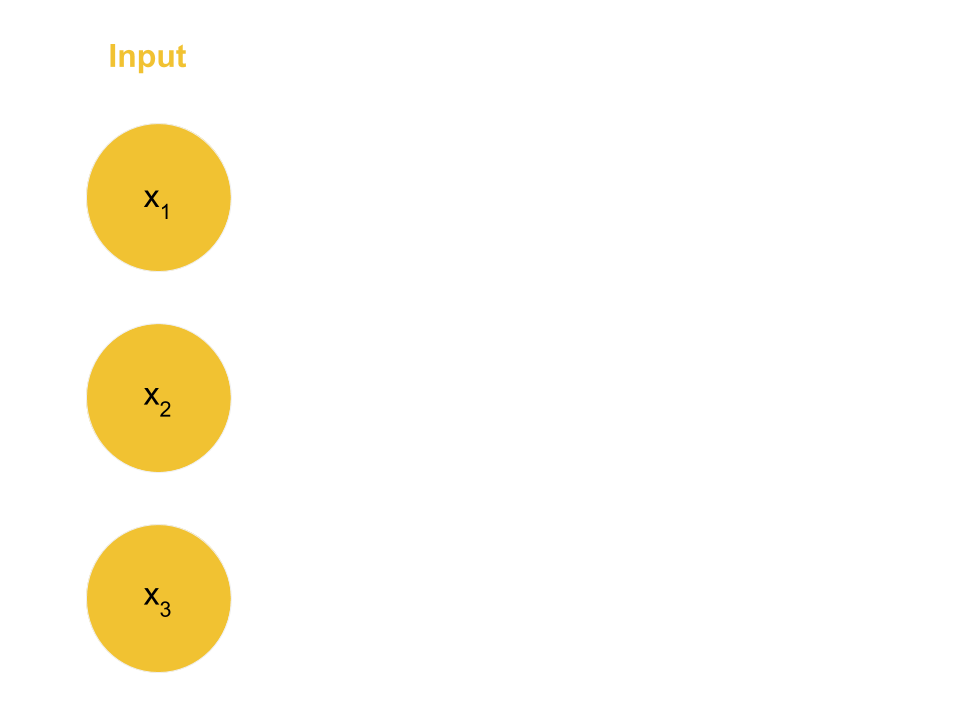
\includegraphics{plots/neurep_one.png}}
  \end{figure}
    \item In general, a $p$-dimensional input vector $\xv$ will be represented by $p$ nodes in the input layer.
  \end{itemize}
\end{frame}

\begin{frame} {A Single Neuron}

We consider a logistic regression model for $p = 3$, i.e. $f(\xv) = \tau(w_1\textcolor{red}{x_1} + w_2\textcolor{red}{x_2} + w_3\textcolor{red}{x_3} + b)$.

  \begin{itemize}
    \item Next, weights $\mathbf{w}$ are represented by edges from the input layer.
    \begin{figure}
    \centering
      \scalebox{0.7}{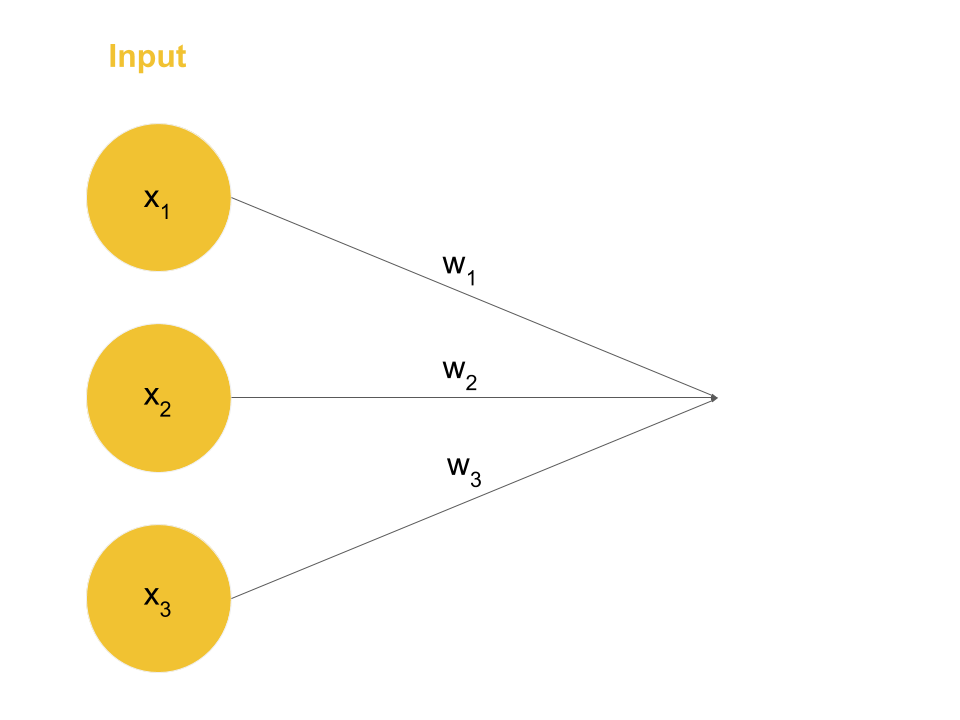
\includegraphics{plots/neurep_two.png}}
  \end{figure}
    \item The bias term $b$ is implicit. It is not shown/represented visually.
  \end{itemize}
\end{frame}

\begin{frame}{A Single Neuron}

\textbf{Note:} For an explicit graphical representation of the bias term, we can do a simple trick: 

\begin{itemize}
  \item we add a constant feature to the inputs $\tilde{\xv} = (1, x_1, ..., x_p)^\top$
  \item and the bias term to the weight vector $\tilde{\bm{w}} = (b, w_1, ..., w_p)$.
\end{itemize}

The graphical representation is then: 

\vspace*{-0.1cm}

\begin{figure}
\scalebox{0.60}{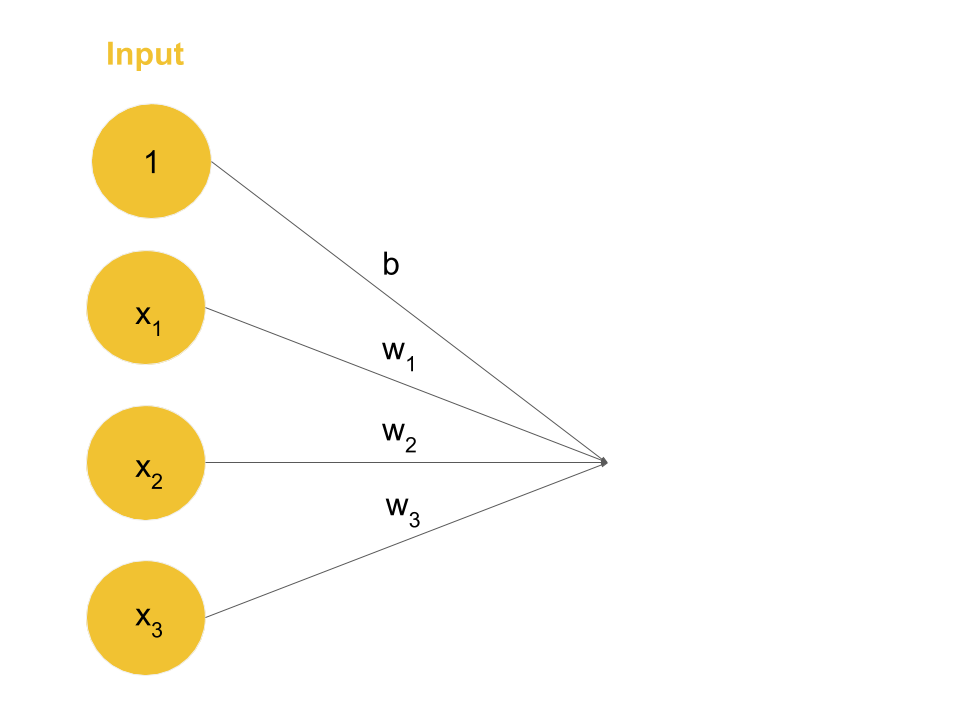
\includegraphics{plots/neurep_bias.png}}
            \caption{Weights and bias of the neuron.}
\end{figure}

\end{frame}

\begin{frame} {A Single Neuron}

We consider a logistic regression model for $p = 3$, i.e. $f(\xv) = \tau(w_1\textcolor{red}{x_1} + w_2\textcolor{red}{x_2} + w_3\textcolor{red}{x_3} + b)$.

  \begin{itemize}
    \item Finally, the computation $\tau(w_1x_1 + w_2x2 + w_3x_3 + b)$ is represented by the neuron in the \enquote{output layer}.
    \begin{figure}
    \centering
      \scalebox{0.7}{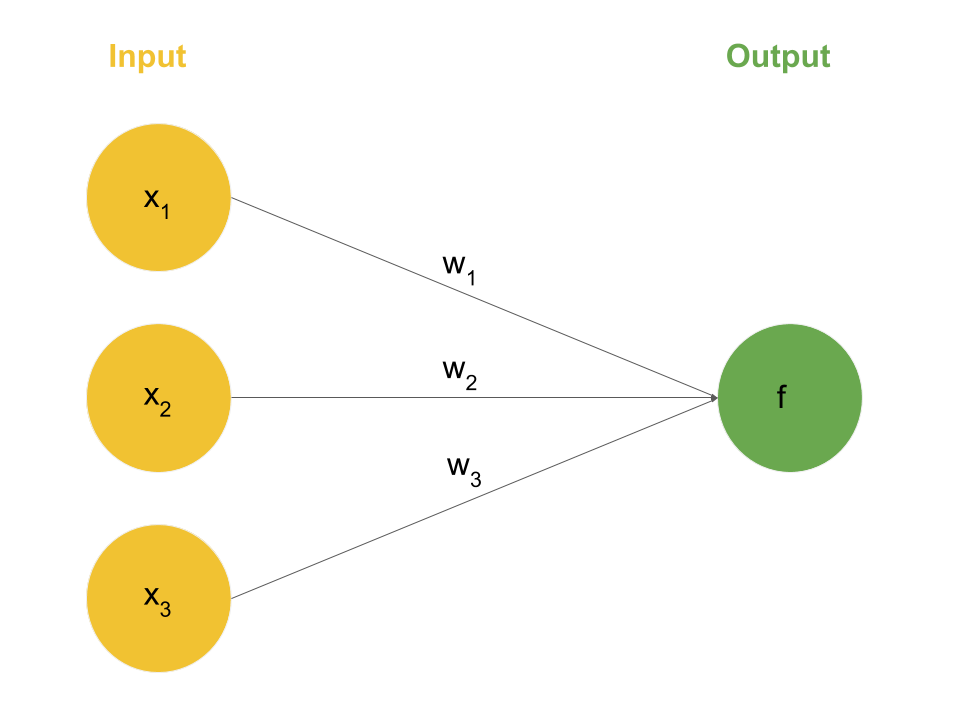
\includegraphics{plots/neurep_three.png}}
  \end{figure}
  \end{itemize}
  \vspace*{-0.5cm}
    \small{Because this single neuron represents exactly the same hypothesis space as logistic regression, it can only learn linear decision boundaries.}
\end{frame}



\begin{frame} {A Single Neuron}
  \begin{itemize}
    \item Therefore, a neuron is just a graphical representation of a very specific kind of function.
    \vspace{4mm}
    \item Every neuron performs a 2-step computation:
      \begin{itemize}
        \item Step 1: compute the weighted sum of inputs (with bias).
        \item Step 2: apply an \textbf{activation function} to the sum,  which is usally  a non-linear transformation of the input.
      \end{itemize}
    \vspace{4mm}
    \item With a single neuron, the activation function serves to constrain the output to the desired range of values. In case of logistic regression. For example, it squashes the output into $[0, 1]$. 
    \vspace{4mm}
    \item However, we will see that activation functions serve a far more important purpose. They are one of the main reasons that neural networks can represent extremely complicated functions.
  \end{itemize}
\end{frame}

\begin{frame} {A Single Neuron}
  \begin{itemize}
    \item \small{One very nice thing about the graphical representation of the function is that you can picture the input vector being "fed" to the neuron on the left followed by a sequence of computations being performed from left to right. This is called a \enquote{\textbf{forward pass}}}.
  \end{itemize}
  \begin{figure}
    \centering
      \only<1>{\scalebox{0.70}{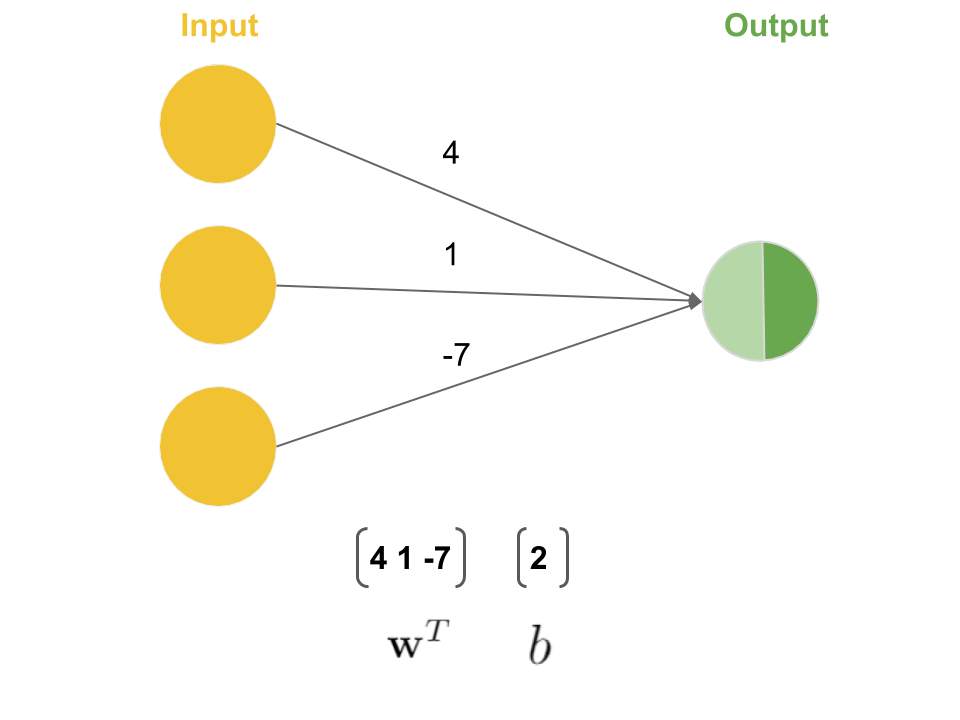
\includegraphics{plots/neuron_one.png}}
            \caption{Weights (and bias) of the neuron.}}
      \only<2>{\scalebox{0.70}{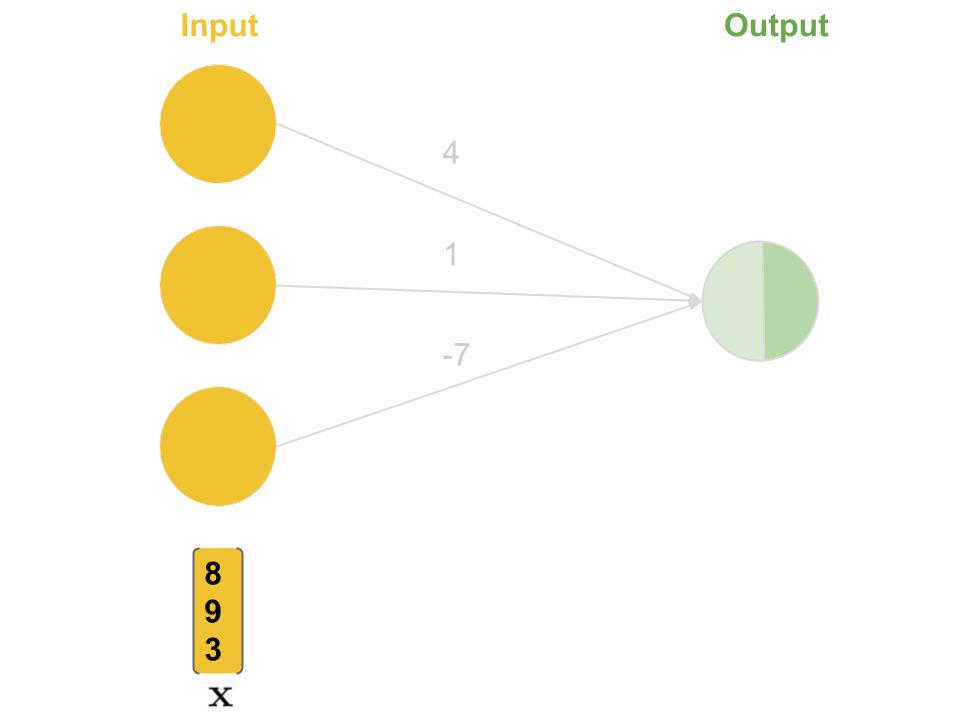
\includegraphics{plots/neuron_two.png}}      \caption{Feed the input on the left.}}
      \only<3>{\scalebox{0.70}{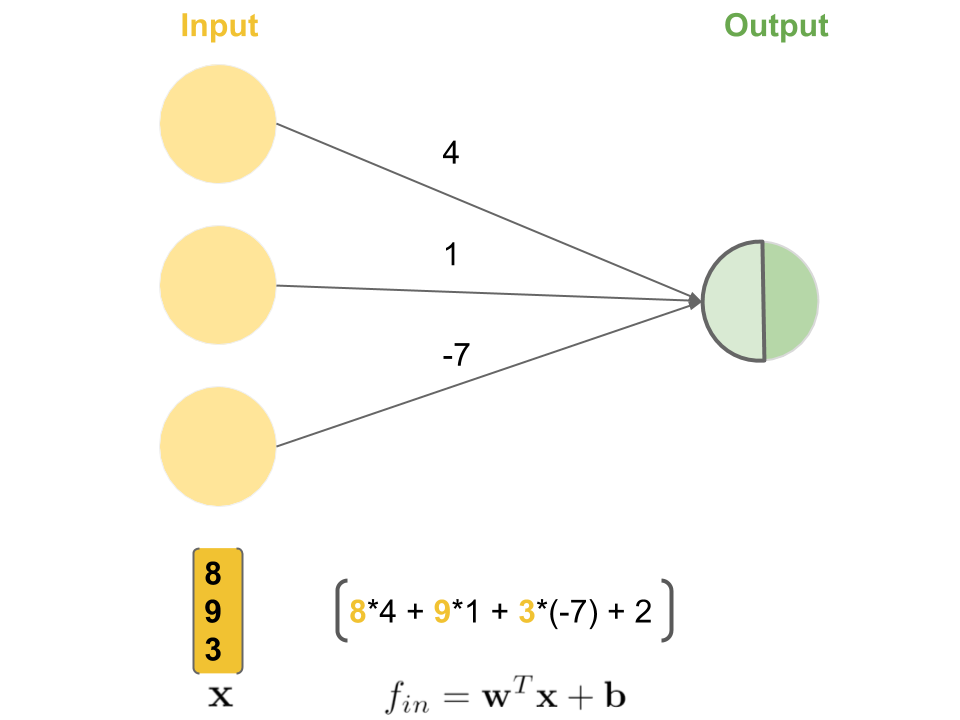
\includegraphics{plots/neuron_three.png}}\caption{Step 1: Compute the weighted sum.}}
      \only<4>{\scalebox{0.70}{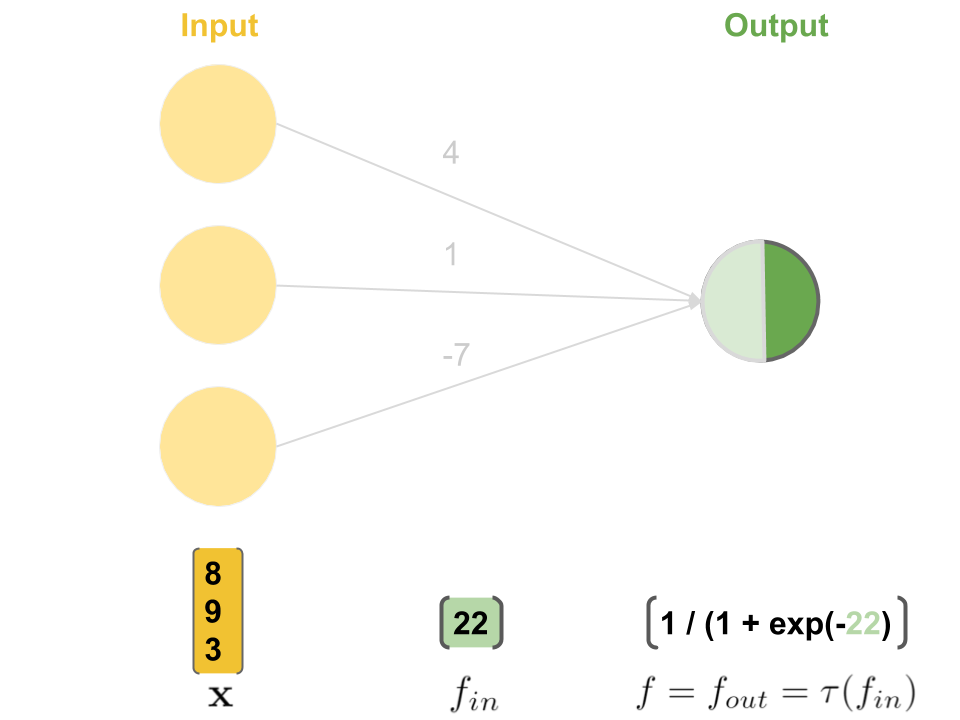
\includegraphics{plots/neuron_six.png}} \caption{Step 2: Apply the activation function.}}
      \only<5>{\scalebox{0.70}{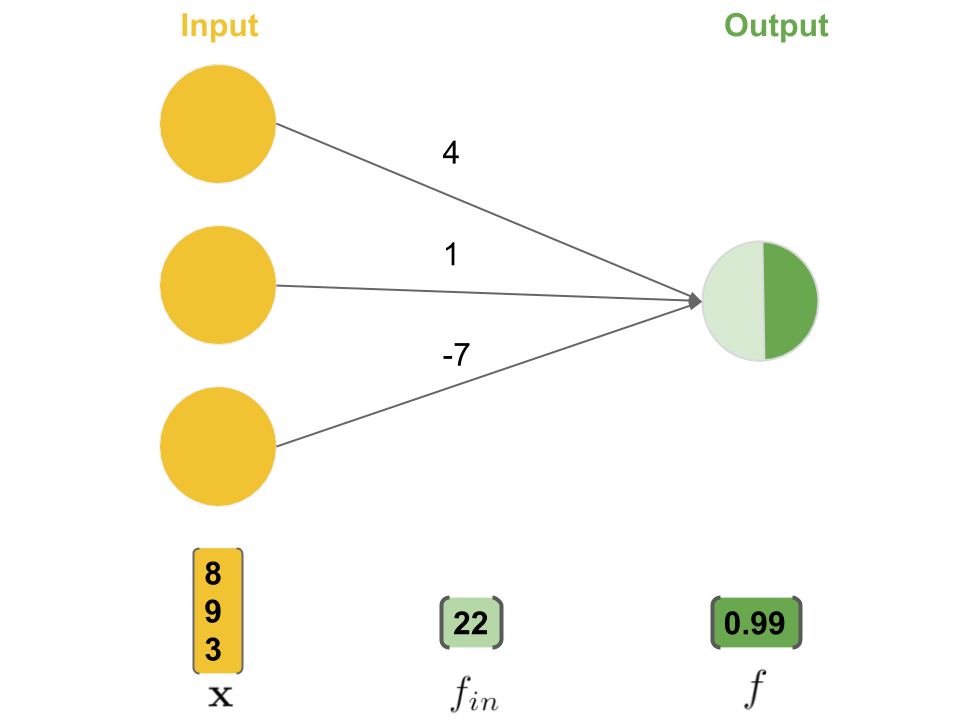
\includegraphics{plots/neuron_seven.png}}}
  \end{figure}
\end{frame}

\begin{frame} {A Single Neuron}
  \begin{itemize}
    \item \small{Even though all neurons compute a weighted sum in the first step, there is considerable flexibility in the type of activation function used in the second step.
    \item For example, setting the activation function to the identity function allows a neuron to represent linear regression.}
  \begin{figure}
    \centering
      \scalebox{0.70}{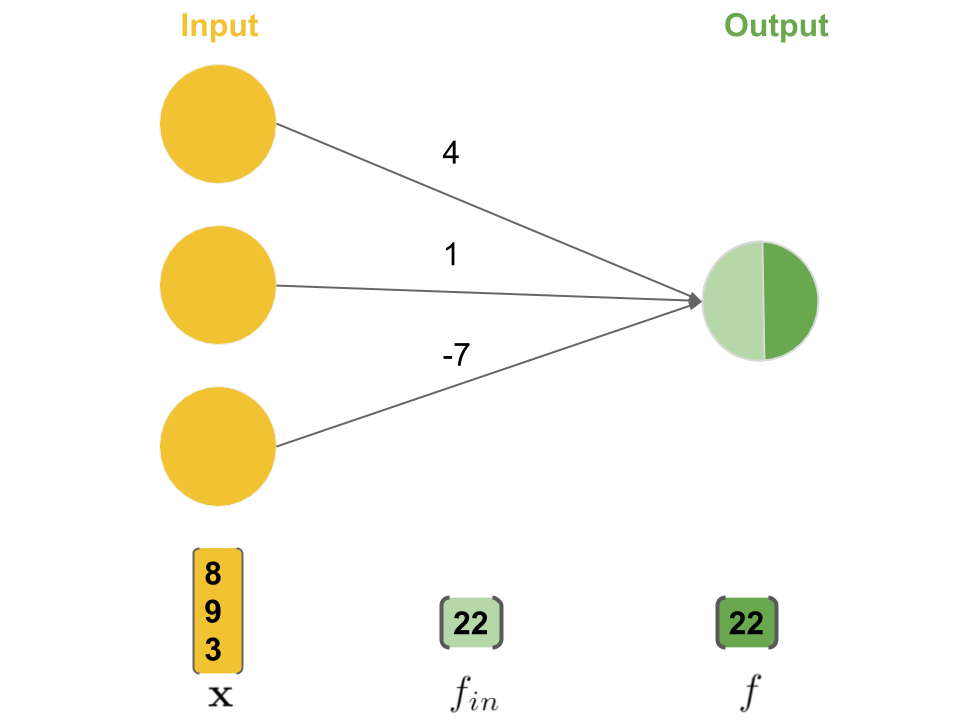
\includegraphics{plots/neuron_five.png}}
  \end{figure}  \end{itemize}
\end{frame}

\begin{vbframe}{A Single Neuron}
  
\begin{itemize}
  \item The hypothesis space that is formed by single neuron architectures is 
  \begin{small}
    $$
      \Hspace  = \left\{f: \R^p \to \R ~\bigg|~ \fx = \tau\left(\sum_{j = 1}^p w_j x_j + b\right), \wtw \in \R^p, b \in \R\right\}.
    $$ 
  \end{small}
  \item Both logistic regression and linear regression are subspaces of $\Hspace$ (if $\tau$ is the logistic sigmoid / identity function).  
\end{itemize}

\vspace*{-0.48cm}

\begin{figure}
  \centering
    \scalebox{0.9}{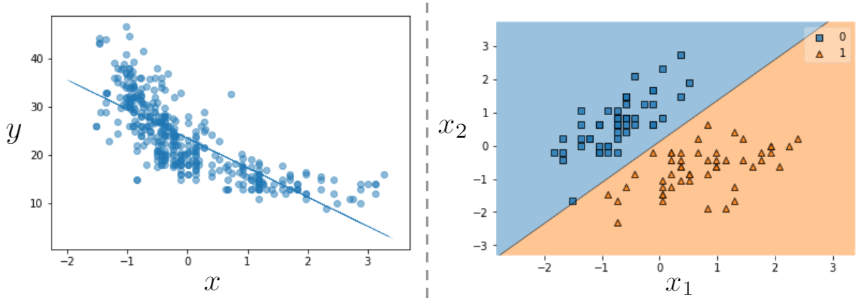
\includegraphics{plots/neuron_regcls.png}}
    \vspace*{-0.2cm}
    \begin{tiny}
    \caption{\textit{Left}: A regression line learned by a single neuron. \textit{Right}: A decision-boundary learned by a single neuron in a binary classification task.}
    \end{tiny}
\end{figure}

\end{vbframe}


\begin{vbframe} {A Single Neuron: Optimization}
  \begin{itemize}
    \item   
    To optimize this model, we minimize the empirical risk 

    $$
      \riske = \sumin \Lxyi, 
    $$

    where $\Lxy$ is a loss function. It compares the network's predictions $\fx$ to the ground truth $y$. 
    \item For regression, we typically use the L2 loss (rarely L1): $$\Lxy = \frac{1}{2}(y - \fx)^2$$
    \item For binary classification, we typically apply the cross entropy loss (also known as bernoulli loss): 
     $$\Lxy = y \log \fx + (1 - y) \log(1 - \fx)$$
    
    \framebreak 

    \item For a single neuron, in both cases, the loss function is convex and the global optimum can be found with an iterative algorithm like gradient descent. 

    \item In fact, a single neuron with logistic sigmoid function trained with the bernoulli loss does not only have the same hypothesis space as a logistic regression and is therefore the same model, but will also yield to the very same result when trained until convergence.
  \end{itemize}
\end{vbframe} 

\endlecture 
\end{document}